\documentclass[french]{article}
\usepackage{verbatim}
\usepackage{amsmath,amsfonts,amssymb}
\usepackage{pgfplots}
\usepackage[utf8]{inputenc}
\usepackage[french]{babel}
\usepackage{pgf,tikz,tkz-tab}
\usepackage{mathrsfs}
\usetikzlibrary{arrows}
\usepackage{pstricks}
\pgfplotsset{compat=newest}
\usepackage{geometry}
\usepackage{eurosym}
\geometry{hmargin=2cm,vmargin=2cm}


\begin{document}

Nom: \\

Prénom:

\begin{center}
\section*{Devoir surveillé IV} 
\textit{Le sujet est à rendre avec la copie, la partie ensemble de nombre et distance est à faire directement sur la feuille et la partie problème sur une copie double.}
\end{center}

\section*{Ensemble de nombre et distance}

1) Compléter le nom des ensembles suivants et rappeler les définitions des ensembles suivants ou le symbole correspondant à cet ensemble: \\

l'ensemble des entiers ....

$\mathbb{N}=$ \\

l'ensemble des entiers ....

$\mathbb{Z}=$ \\

l'ensemble des nombres .....

$\{ \frac{a}{10^n} / a \in \mathbb{Z}, n \in \mathbb{N} \}=$ \\


l'ensemble des nombres .....

$\{ \frac{a}{b} / a \in \mathbb{Z}, b \in \mathbb{N}^* \}=$ \\

2) Donner un élément qui appartient à $\mathbb{Z}$ et qui n'appartient pas à $\mathbb{N}$. \\

3) Donner un élément qui appartient à $\mathbb{R}$ et qui n'appartient pas à $\mathbb{Q}$.\\



4) Pour chaque cas, compléter la phrase puis tracer une représentation de la droite des réels et représenter chaque intervalle sur celle-ci. \\



Si $ 2 \leq x \leq 6 $ cela équivaut à dire que $x$ appartient à l'intervalle .... \\

	\vspace{0.5cm}

Si $ -2 \leq x < 3 $ alors cela équivaut à dire que $x$ appartient à l'intervalle .... \\

  \vspace{0.5cm}
  
  Si $ 4 \geq x > 3 $ alors cela équivaut à dire que $x$ appartient à l'intervalle .... \\

  \vspace{0.5cm}

  Si $ x \geq 3 $ alors cela équivaut à dire que $x$ appartient à l'intervalle .... \\
  
  \vspace{0.5cm}


5) Soit $r \in \mathbb{R}_{+}^*$ alors $ \vert x \vert \leq r $ équivaut à l'inégalité  $ ... \leq x \leq ... $.

 Si $  \vert x - 5 \vert \leq 7 $ alors cela équivaut à dire que $x$ est à une distance de $5$ ..... ou égale à $7$, on peut dire que $x$ appartient à l'intervalle .... \\

(BONUS 1 point)  Si $  \vert x - 1 \vert > 2 $ , on peut dire que $x$ appartient à l'intervalle .... \\

\newpage

 
\section*{Problème}

\subsection*{Rappel de géométrie}

Soit un triangle équilatéral $T$ de coté $x \in \mathbb{R}_{+}^{*}$, pour le moment, l'objectif est de calculer l'aire d'un triangle équilatéral à partir de la longueur d'un de ces cotés. \\

\begin{center}
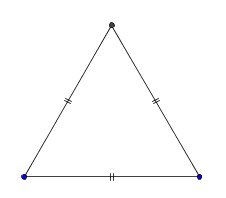
\includegraphics[scale=1]{equi3.png}
\end{center}


On rappel que la hauteur d'un triangle équilatéral est aussi la médiane. On obtient ainsi la figure suivante. \\

6) Déterminer $A_T$, l'aire  de $T$ en fonction de $x$.

On posera maintenant $A_T=\frac{\sqrt{3} \times x^2}{4}$.

\subsection*{Triangle de Sierpiński}

Le triangle de Sierpiński, est une fractale, du nom de Wacław Sierpiński.\\

\begin{center}
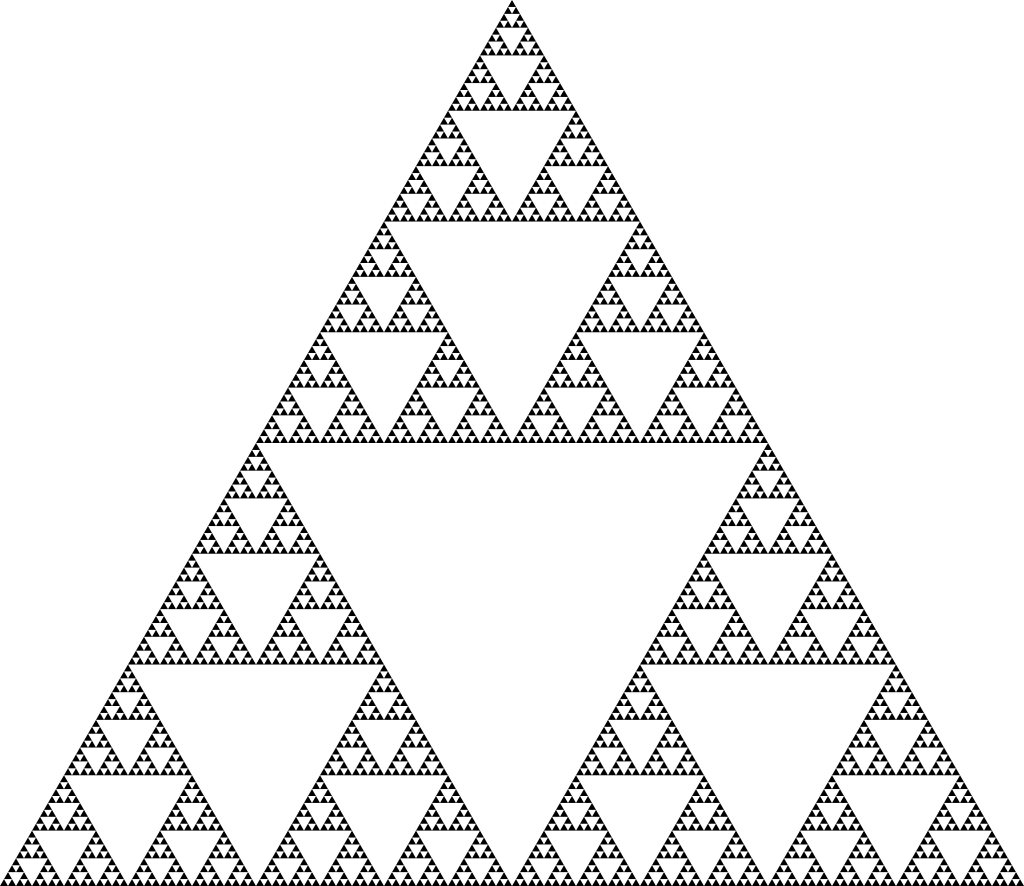
\includegraphics[scale=0.15]{sier.png}
\end{center}

Il peut s'obtenir à partir d'un triangle équilatéral « plein » , par une infinité de répétitions consistant à diviser par deux la taille du triangle puis à les accoler en trois exemplaires par leurs sommets pour former un nouveau triangle. À chaque répétition le triangle est donc de même taille, mais « de moins en moins plein ».

\begin{center}
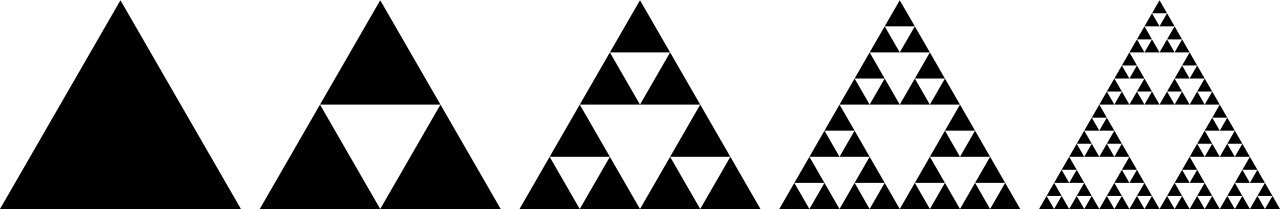
\includegraphics[scale=0.15]{sier2.png}
\end{center}


Soit ici un triangle équilatéral de coté $x \in \mathbb{R}_{+}^{*}$

On note $A_{T_1}$ l'aire \underline{d'un seul triangle plein} formés lors de la \underline{première itération}. \emph{(voir ci-dessus)}\\


7) Déterminer $A_T$ en fonction de $A_{T_1}$.

8) En déduire alors $A_{T_1}$ en fonction de $x$.

9) Déterminer le nombre de triangle plein en fonction du nombre d'itération noté $n$.

10) Déterminer la bonne longueur de $x$ pour que l'aire des triangles plein de la première itération soit égale à 1.



\end{document}

